\documentclass[a4paper,12pt]{article}
\usepackage[slovene]{babel}
\usepackage[utf8]{inputenc}
\usepackage[T1]{fontenc}
\usepackage{lmodern}

\usepackage{url}
\usepackage{graphicx}
\usepackage{xcolor}
\usepackage{amsmath}
\usepackage{amsthm}
\usepackage{amssymb}

\usepackage{booktabs}

\setlength{\belowcaptionskip}{2mm}
\setlength{\parindent}{0mm}

\newcommand{\m}{\mathcal{M}_2}
\newcommand{\pojem}[1]{\emph{\color{purple}#1}}

\theoremstyle{definition}
\newtheorem{definicija}{Definicija}

\theoremstyle{plain}
\newtheorem{izrek}{Izrek}


\newenvironment{dokaz}{%
	\begin{proof}[Dokaz izreka]%
}{%
	\end{proof}%
}

\newenvironment{magic}[3]
{
   \begin{table}[!ht]
      \centering
      \caption{#2}
      \label{#3}
      \large
      \begin{tabular}{|*{#1}{c|}}
      \hline
}
{
      \end{tabular}
      \normalsize
   \end{table}
}

\title{Magični kvadrati}
\author{}
\date{}

\begin{document}

%%%%%%%%%%%%%%%%%%%%%%%%%%%%%%%%%%%%%%%%%%%%%%%%%%%%%%%%%%%%%%%%%%%%%%%%

\maketitle

\begin{center}
   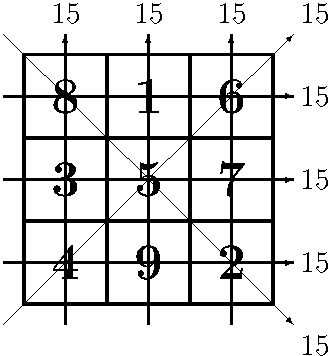
\includegraphics{slika.pdf}
\end{center}

Prirejeno iz virov:
%
\begin{itemize}
   \item \url{http://mathworld.wolfram.com/MagicSquare.html}
   \item \url{http://en.wikipedia.org/wiki/Magic_square}
\end{itemize}

\tableofcontents

%%%%%%%%%%%%%%%%%%%%%%%%%%%%%%%%%%%%%%%%%%%%%%%%%%%%%%%%%%%%%%%%%%%%%%%%

\newpage

\section{Uvod}

\begin{definicija}
   \pojem{Magični kvadrat} reda $n$ je nabor $n^2$ različnih števil,
   ki so razvrščena v kvadratno tabelo tako, da vedno dobimo enako vsoto,
   če seštejemo vsa števila poljubne vrstice, vsa števila poljubnega
   stolpca ali vsa števila v katerikoli od glavnih diagonal.
\end{definicija}

Primer magičnega kvadrata reda 3 je prikazan v tabeli~\ref{table:mag3}.

\begin{magic}{3}{Magični kvadrat reda 3}{table:mag3}
   8 & 1 & 6 \\\hline
   3 & 5 & 7 \\\hline
   4 & 9 & 2 \\\hline
\end{magic}

\begin{definicija}
   Magični kvadrat reda $n$ je \pojem{normalen}, če v njem nastopajo števila
   \begin{equation}
      \label{eq:numbers}
      1, 2, 3, \ldots, n^2-1, n^2.
   \end{equation}
\end{definicija}

Magični kvadrat v tabeli \ref{table:mag3} je normalen.
To je tudi najmanjši netrivialen normalen magični kvadrat.
Poleg normalnih magičnih kvadratov so zanimivi tudi magični kvadrati praštevil.

%%%%%%%%%%%%%%%%%%%%%%%%%%%%%%%%%%%%%%%%%%%%%%%%%%%%%%%%%%%%%%%%%%%%%%%%

\section{Zgodovina}

\subsection{Kvadrat ">Lo Shu"<}

Kitajska literatura iz časa vsaj 2800 let pred našim štetjem govori o legendi
\pojem{Lo Shu} -- ">zvitek reke Lo"<. V antični Kitajski je prišlo do
silne poplave. Ljudje so skušali rečnemu bogu narasle reke Lo ponuditi daritev,
da bi pomirili njegovo jezo. Iz vode se je prikazala želva z zanimivim vzorcem
na oklepu: v tabeli velikosti tri krat tri so bila predstavljena števila, tako
da je bila vsota števil v katerikoli vrstici, kateremkoli stolpcu in na obeh
glavnih diagonalah enaka: 15. To število je tudi enako številu dni v 24 ciklih
kitajskega sončnega leta. Ta vzorec so na določen način uporabljali upravljalci
reke.

\begin{magic}{3}{Kvadrat Lo Shu}{table:loshu}
   4 & 9 & 2 \\\hline
   3 & 5 & 7 \\\hline
   8 & 1 & 6 \\\hline
\end{magic}

%%%%%%%%%%%%%%%%%%%%%%%%%%%%%%%%%%%%%%%%%%%%%%%%%%%%%%%%%%%%%%%%%%%%%%%%

\subsection{Kulturna pomembnost}

Magični kvadrati so fascinirali človeštvo skozi vso zgodovino. Najdemo jih
v številnih kulturah, npr.\ v Egiptu in Indiji, vklesane v kamen ali
kovino, uporabljane kot talismane za dolgo življensko dobo in v
izogib boleznim.

\pojem{Kubera-Kolam} je talna poslikava, ki se uporablja v Indiji, in je v
obliki magičnega kvadrata reda 3. Ta je v bistvu enak kot kvadrat
Lo Shu, vendar je vsako število povečano za 19.

\begin{magic}{3}{Kvadrat Kubera-Kolam}{table:kubera}
   23 & 28 & 21 \\\hline
   22 & 24 & 26 \\\hline
   27 & 20 & 25 \\\hline
\end{magic}

Z magičnimi kvadrati so se ukvarjali tudi najbolj znani matematiki kot na
primer Euler, glej \cite{euler}.

%%%%%%%%%%%%%%%%%%%%%%%%%%%%%%%%%%%%%%%%%%%%%%%%%%%%%%%%%%%%%%%%%%%%%%%%

\subsection{Zgodnji kvadrati reda 4}

Najzgodnejši znani magični kvadrat reda 4 je bil odkrit na napisu
v Khajurahu v Indiji in v Enciklopediji Bratovščine Čistosti iz enajstega
ali dvanajstega stoletja. Vrh vsega gre celo za ">panmagični kvadrat"<.
V Evropi sta morda najbolj znana naslednja magična kvadrata reda 4.

\paragraph{Magični kvadrat v litografiji Melancholia I}
(glej sliko \ref{fig:durer}
za izsek s kvadratom) Albrechta Dürerja naj bi bil najzgodnejši magični kvadrat
v evropski umetnosti. Zelo podoben je kvadratu Yang Huija, ki je nastal na Kitajskem
približno 250 let pred Dürerjevim časom.
%
\begin{figure}[!ht]
   \centering
   \caption{Dürerjev magični kvadrat}
   \label{fig:durer}
   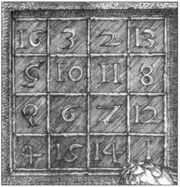
\includegraphics[scale=1.3]{durer.png}
\end{figure}

Vsoto 34 je mogoče najti pri seštevanju števil v vsaki vrstici, vsakem stolpcu,
na vsaki diagonali, v vsakem od štirih kvadrantov, v sredinskih štirih poljih,
v štirih kotih, v štirih sosedih kotov v smeri urinega kazalca ($3+8+14+9$), v
štirih sosedih kotov v nasprotni smeri urinega kazalca ($2+5+15+12$), v dveh naborih
simetričnih parov ($2+8+9+15$ in $3+5+12+14$), in še na nekaj drugih načinov.
Števili na sredini spodnje vrstici tvorita letnico litografije: 1514.
%
\begin{magic}{4}{Dürerjev magični kvadrat $4\times 4$}{table:durer}
   16 &  3 &  2 & 13 \\\hline
    5 & 10 & 11 &  8 \\\hline
    9 &  6 &  7 & 12 \\\hline
    4 & 15 & 14 &  1 \\\hline
\end{magic}

\paragraph{Pasijonska fasada na katedrali Sagrada família v Barceloni}
(glej sliko \ref{fig:sagrada} za fotografijo) vsebuje magični kvadrat reda 4.
%
\begin{figure}[!ht]
   \centering
   \caption{Pasijonska fasada, Sagrada Família}
   \label{fig:sagrada}
   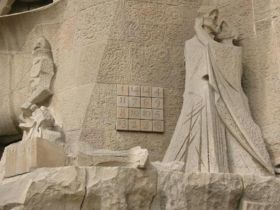
\includegraphics[scale=0.45]{sagrada.png}
\end{figure}

Vsota števil v vrsticah, stolpcih oziroma na diagonalah je 33 -- Jezusova starost
v času pasijona. Strukturno je kvadrat podoben Dürerjevemu, vendar so števila
v štirih poljih zmanjšana za 1. Posledica je, da sta števili 10 in 14 podvojeni
in zato kvadrat ni normalen.
% 
\begin{magic}{4}{Magični kvadrat na Sagradi Famíliji}{table:sagrada}
   1 & 14 & 14 &  4 \\\hline
  11 &  7 &  6 &  9 \\\hline
   8 & 10 & 10 &  5 \\\hline
  13 &  2 &  3 & 15 \\\hline
\end{magic}

%%%%%%%%%%%%%%%%%%%%%%%%%%%%%%%%%%%%%%%%%%%%%%%%%%%%%%%%%%%%%%%%%%%%%%%%

\section{Osnovne lastnosti}

\begin{definicija}
   Vsoto ene vrstice, enega stolpca ali ene od glavnih diagonal
   v magičnem kvadratu imenujemo \pojem{magična konstanta}.
\end{definicija}

\begin{izrek}
   Magična konstanta normalnega magičnega kvadrata reda $n$
   je enaka
   \begin{equation}
      \label{eq:mc}
      \m(n) = \frac{1}{2} n(n^2+1).
   \end{equation}
\end{izrek}

\begin{dokaz}
   V normalnem magičnem kvadratu reda $n$ je vsota vseh nastopajočih
   števil (glej \eqref{eq:numbers} na strani \pageref{eq:numbers}) enaka
   $1+2+3+\dots+n^2=\sum_{k=1}^{n^2}k=\frac{1}{2}n^2(n^2+1)$. Ker imamo
   v kvadratu $n$ vrstic z enako vsoto, je vsota števil v eni vrstici
   enaka številu $\m(n)$.
\end{dokaz}

Preprost račun pokaže, da je konstanti \eqref{eq:mc} analogna konstanta
$\m(n;A,D)$ za magični kvadrat, v katerem so nameščena števila
$A$, $A+D$, $A+2D$, \dots, $A+(n^2-1)D$, enaka
\[
   \m(n;A,D) = \frac{1}{2} n \left(2A+D(n^2-1)\right).
\]
Kvadratu v tabeli \ref{table:kubera} ustrezata konstanti $A=20$ in $D=1$.

\begin{definicija}
   Če vsako od števil v normalnem magičnem kvadratu reda $n$ odštejemo
   od števila $n^2+1$, dobimo nov magični kvadrat, ki je prvotnemu
   \pojem{komplementaren}.
\end{definicija}

Na primer, magičnemu kvadratu Lo Shu (glej tabelo \ref{table:loshu}) priredimo
komplementarni kvadrat, prikazan v tabeli \ref{table:closhu}.

\begin{magic}{3}{Kvadratu Lo Shu komplementarni kvadrat}{table:closhu}
   6 & 1 & 8 \\\hline
   7 & 5 & 3 \\\hline
   2 & 9 & 4 \\\hline
\end{magic}

Vidimo, da je dobljeni kvadrat moč dobiti iz kvadrata Lo Shu tudi z zasukom za
180 stopinj okrog središča, kvadrat iz tabele \ref{table:mag3} pa je mogoče dobiti
iz kvadrata Lo Shu z zrcaljenjem preko sredinske vodoravne črte.

\begin{definicija}
   Pravimo, da sta dva magična kvadrata \pojem{različna}, če enega ni mogoče dobiti
   iz drugega s pomočjo zasukov oziroma zrcaljenj.
\end{definicija}

Števila različnih normalnih magičnih kvadratov se nahajajo v tabeli \ref{table:stevila}.

\begin{table}[!ht]
   \centering
   \caption{Število različnih normalnih magičnih kvadratov}
   \label{table:stevila}
   \begin{tabular}{lcccccc}\toprule
      & \multicolumn{5}{c}{točna vrednost} & približek \\
      \midrule
      red & 1 & 2 & 3 & 4 & 5 & 6 \\
      število kvadratov & 1 & 0 & 1 & 880 & 275305224 & $(1{,}7745 \pm 0{,}0016)10^{19}$ \\
      % TODO: siunitx (poglej pri Bauerju, tabele.tex)
      \bottomrule
   \end{tabular}
\end{table}

Vse normalne magične kvadrate reda 4 je oštevilčil Frénicle de Bessy
leta 1693, glej \cite{bessy}, in jih je moč najti v knjigi \cite{berlekamp}
iz leta 1982. Število normalnih kvadratov reda 5 je izračunal
R. Schroeppel leta 1973 (glej Gardner \cite{gardner}).
Natančno število vseh različnih normalnih magičnih kvadratov reda 6 ni znano.
Avtorja navedenega približka sta Pinn in Wieczerkowski (glej \cite{pinn}), ki
sta za oceno uporabila simulacijo Monte Carlo in metode statistične mehanike.

%%%%%%%%%%%%%%%%%%%%%%%%%%%%%%%%%%%%%%%%%%%%%%%%%%%%%%%%%%%%%%%%%%%%%%%%

\section{Primeri}

V tabelah \ref{table:mag5}, \ref{table:mag6} in \ref{table:mag9} so prikazani
magični kvadrati redov 5, 6 in 9.

\begin{magic}{5}{Magični kvadrat reda 5}{table:mag5}
   17 & 24 &  1 &  8 & 15 \\\hline
   23 &  5 &  7 & 14 & 16 \\\hline
    4 &  6 & 13 & 20 & 22 \\\hline
   10 & 12 & 19 & 21 &  3 \\\hline
   11 & 18 & 25 &  2 &  9 \\\hline
\end{magic}

\begin{magic}{6}{Magični kvadrat reda 6}{table:mag6}
    6 & 32 &  3 & 34 & 35 &  1 \\\hline
    7 & 11 & 27 & 28 &  8 & 30 \\\hline
   19 & 14 & 16 & 15 & 23 & 24 \\\hline
   18 & 20 & 22 & 21 & 17 & 13 \\\hline
   25 & 29 & 10 &  9 & 26 & 12 \\\hline
   36 &  5 & 33 &  4 &  2 & 31 \\\hline
\end{magic}

\begin{magic}{9}{Magični kvadrat reda 9}{table:mag9}
   47 & 58 & 69 & 80 &  1 & 12 & 23 & 34 & 45 \\\hline
   57 & 68 & 79 &  9 & 11 & 22 & 33 & 44 & 46 \\\hline
   67 & 78 &  8 & 10 & 21 & 32 & 43 & 54 & 56 \\\hline
   77 &  7 & 18 & 20 & 31 & 42 & 53 & 55 & 66 \\\hline
    6 & 17 & 19 & 30 & 41 & 52 & 63 & 65 & 76 \\\hline
   16 & 27 & 29 & 40 & 51 & 62 & 64 & 75 &  5 \\\hline
   26 & 28 & 39 & 50 & 61 & 72 & 74 &  4 & 15 \\\hline
   36 & 38 & 49 & 60 & 71 & 73 &  3 & 14 & 25 \\\hline
   37 & 48 & 59 & 70 & 81 &  2 & 13 & 24 & 35 \\\hline
\end{magic}

\newpage

%%%%%%%%%%%%%%%%%%%%%%%%%%%%%%%%%%%%%%%%%%%%%%%%%%%%%%%%%%%%%%%%%%%%%%%%

\bibliographystyle{siam}
\bibliography{magic}

\end{document}
